\section{Project overview}


\subsection{Aim and purpose}
This project is intended to give knowledge and experience in design and fabrication of CMOS VLSI chips. This includes:
\begin{enumerate}
 \item Deep insight in physical design of VLSI chips.
 \item Knowledge and experience of using professional CAD tools for design, simulation, layout, and verification of VLSI chips.
 \item Design of a ‘real’ and functional chip, starting from the idea and behavioral modeling to detailed circuit design at transistor level, circuit layout, and final verifications.
 \item Complete the project using a systematic and professional approach required by industry to run large and complex VLSI projects.
\end{enumerate}

\subsection{System overview}
The following block diagram taken directly from the requirements specification illustrates system that shall be implemented.
\begin{figure}[H]
  \begin{center}
    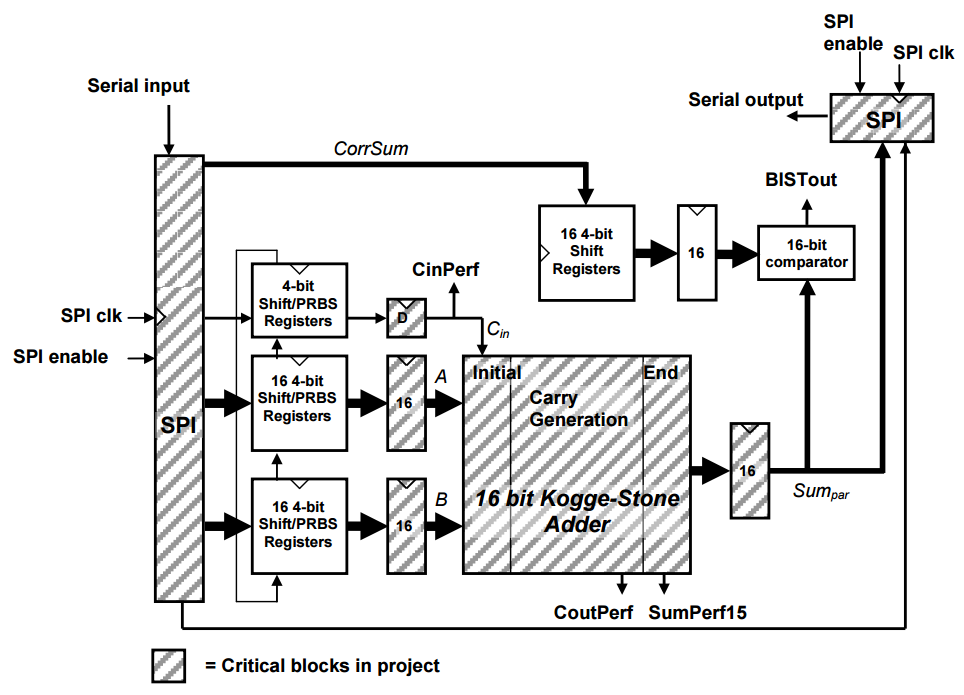
\includegraphics[keepaspectratio=true,width=375px]{grafik/block.png}
    \caption{System block diagram of adder and evaluation circuitry}
    \label{organisationsplan}
  \end{center}
\end{figure}